How exactly are microorganisms supposed to be classified? Is there a consensus in the microbiological community about a methodology considered optimal to classify between microorganisms? The short answer is no. Microorganisms are notoriously difficult to classify, primarily because so little is known about them in the first place per lack of adequate tools and sensors to characterize them \cite{Hutchins2019}, and per the huge amount of time currently required to study them. \par

Any system of scientific classification or cataloguing of things lies under the assumption that there exist an order or system of similarities in nature which can be attained by investigation \cite{Sneath1957}. The science of classification exists to quantify how much a given object A is more or less similar to a second object B than a third object C, and then strives to group these objects accordingly. Now, one first logical way to do this would be to inquire upon the tangible features of an object and group it with other objects that present these very same features \cite{Sneath1957}. But then another challenge arises: how are we to weight these features? In other words, how do these features correlate with members of a same group? Since that knowledge is unknown a priori, classification becomes a problem of correlating features present in certain objects then creating groups that are thought to fit the known objects at the time, then updating the groups and the weights when confronted with conflicting additional data. \par

For animals, some features might be easily discarded. For instance, the weight, the height, the color, the sex, etc. tell us nothing to discriminate between species: this is because those properties are uncorrelated; their knowledge does not lead to any other features of the animal \cite{Sneath1957}. From this example, it is obvious that some features are more important than others, but how can this be applied to classification in microbiology, which is still a relatively new science? Can such features as the size, morphology, composition of the membrane, color, sexual lifecycle, metabolic lifecycle, interaction with substrates, composition of the cytoplasm, presence of specific proteins or lipids, motility, or behavior be considered more important than others? Because before having proved that any feature is more important, their weights should be initialized equally \cite{Sneath1957}. With that in mind, let’s have a better look at how exactly microorganisms will be defined in this study. \par
\begin{figure}[ht]
    \centering
    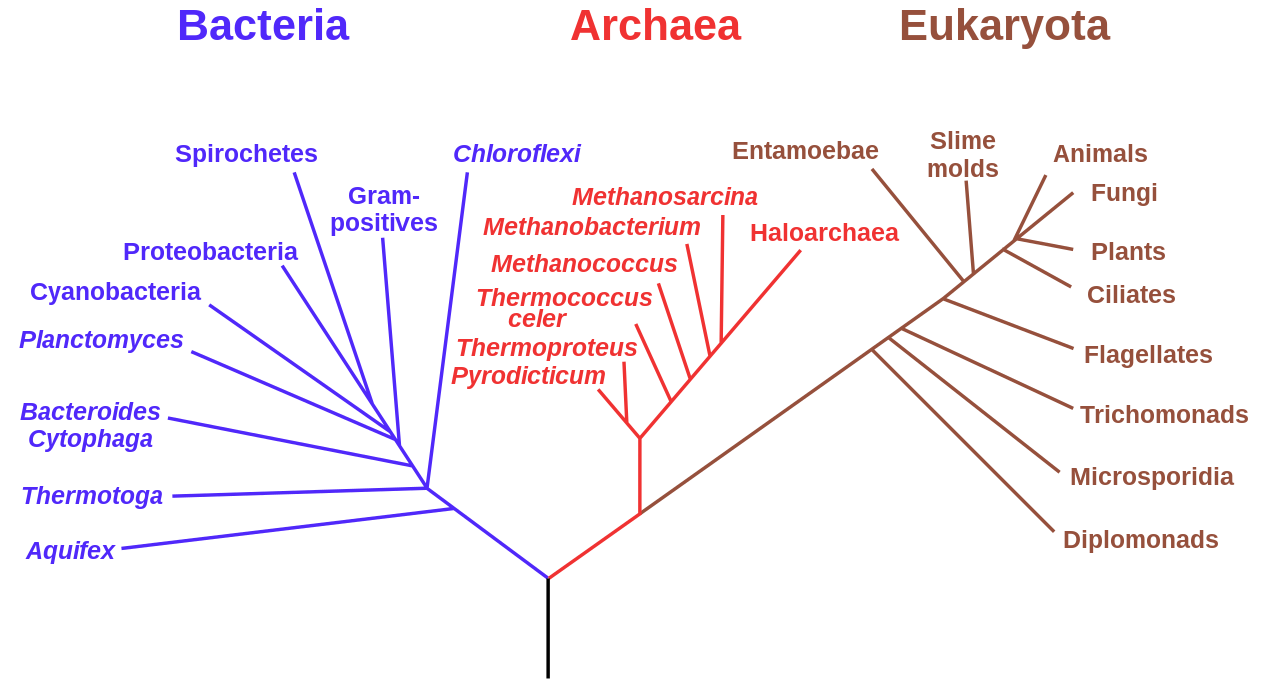
\includegraphics[width=1\textwidth]{DomainsLife}
    \caption{The 3-domains of life featuring Bacteria, Archae and Eukaryota. System of classification proposed by Carl Woese of the University of Illinois in 1990.}
    \label{fig:DomainsLife}
\end{figure}

Microorganisms generally include all living unicellular organisms which cannot be observed with the naked eye. The eyes have trouble distinguishing objects smaller than 200um, meaning that almost all single-celled organisms of the three domains of life are included in this definition. For the purpose of this study, multi-cellular organisms of dimensions below 200um will also be considered as microorganisms. Those include bacteria, archea, fungi, algae, protozoa, plankton, micro-animals such as the subphylum Myxozoa, and members of the Chromista. Those microorganisms inhabit varied environment and are parts of diverse ecosystems which made them evolve extremely diversified features. Hierarchical organization of microorganisms is often found in nature: individuals grouped together form populations (or guilds if they are metabolically related), sets of interacting guilds form communities, and different communities in a specific biotic (macro-organisms such as plants and animals) and abiotic (pH, temperature, inorganic, and organic nutrients) environment form ecosystems \cite{Hutchins2019}. It is by inferring on these varied features and by monitoring the environmental parameters that the microorganisms can be adequately catalogued. Though one practical problem arises for the standardization of tests, as microorganisms thrive in different environmental conditions. Should the tests for different microorganisms be performed at the same environmental conditions, or should they be performed at the optimum thriving condition of the specie? Species behave differently in function of the environmental parameters, and time is lacking to adequately test every specimen under a spectrum of varying environmental conditions. In this case, \citep{cowan1956ordnung} suggested that tests procedure be standardized at a unique environmental condition, since the risk of the tests being unrepeatable seem more important than the risk of the test being vitiated \cite{Sneath1957}. \par

As an example of microorganism cataloguing, bacteria can be differentiated based on the chemical composition of their cell walls. Some bacteria, called Gram-positive, feature a cytoplasmic membrane composed of a lipid bilayer, with a peptidoglycan layer of crosslinked peptides and sugars hidden beneath, beside a large concentration of teichoic acid \cite{Kocanda2014}. Gram-negative bacteria also have a lipid bilayer but have a thinner peptidoglycan layer on top of a second lipid bilayer linked to lipopolysaccharides. Gram-positive bacteria can be observed easily under a scanning electron microscope (SEM) by staining the cell walls with dye. Some bacteria species can be associated with specific chemical structures, like Staphylococcus, Streptococcus, Bacillus, Corynebacteria, Listeria, and Clostridium which all exhibit teichoic acid. The impedance of chemical compounds that compose microorganisms are found to exhibit notable signature that can help in differentiating them. Aliphatic compounds such as lipids and straight-chain alkanes, and organic acids and alcohols that contain ionizable protons are slightly polarizable in unique ways, which make them behave differently under a time-varying electrical fields \cite{Kocanda2014}. Studying these structures is thus found to be primordial to understanding and differentiating microorganisms.\par

A second logical system of classification would be using phylogenetic networks produced on the basis of sequenced genes or genomic data \cite{kapli2020phylogenetic}. This is the most popular system of classification for prokaryote, although it is more of an operational one. Single-cell organisms could be catalogued based on their DNA-DNA re-association. \citep{konstantinidis2005genomic} defines “two strains as being of the same specie when their purified genomic DNA show at least 70\% hybridization, which is equivalent to $94\%$ average nucleotide identity at the whole genome scale”. Species containing similar conserved sequences can then be linked together. Other methods with arbitrary threshold exist. For instance, several studies also define the identity of bacteria from highly conserved prokaryotic genes by sequencing their 16S ribosomal RNA gene (rDNA). Using these universal prokaryotic primers results in reliable and inexpensive taxonomic classification, but favors bacteria over archae, resulting in an under-estimated diversity and taxonomic resolution of archae \cite{Horve2020, Xu2006}. \par

Gene sequencing also suffers from important limitations. Contrarily to what is expected, the networks produced in such manner do not necessarily represent accurately the evolutionary history of the species member. Noise may affect and corrupt the sequencing \cite{kapli2020phylogenetic}. Moreover, the analysis may be troubled by horizontal gene transfer, gene recombination, convergent evolution of similar features, or hybridization between species situated far from each other on the tree. Great care should also be taken when creating phylogenetic trees from a single type of character - such as a protein or gene - since the genomic data represent the phylogeny (history) of that specific character, and not of the whole taxa \cite{kapli2020phylogenetic,Nosenko2013}. Serious phylogenetic studies therefore use data from multiple characters (mitochondrial, nuclear, etc.) from a single taxa in order to reduce the chance of homoplasy (false homology) \cite{kapli2020phylogenetic,Nosenko2013}. All these limitations lead to errors such that common species might be considered separated, or vice-versa. As with any set of data, falsification of previous research might also be induced by more recent studies made with optimized research instruments \cite{kapli2020phylogenetic}. \par

It is important to mention that phylogenetic networks made from genomic data do not translate adequately to the ones used in the animal and plant kingdoms, which are based on common traits. For instance, using it on animals would result in all primates (gorillas, chimpanzees, gibbons, orangutans, and humans) being of the same species \cite{Xu2006}. Instead, the biological species concept is currently the most popular one for sexual organisms possessing a meiotic life cycle, such as the vast majority of plants, animals and sexual eukaryotes. The choice of classification system is still now in evolution, this explains the numerous modifications in the species concepts observed for prokaryote and eukaryote in the scientific community \cite{Xu2006}. \par

The state of the art for scientific classification of prokaryote being phylogenetic networks, grouping microorganisms based on physical features should be called cataloguing, as opposed to proper scientific taxonomy, as it is effectively used only as a parallel approach to find tangible feature-keys for identification \cite{Sneath1957}.